\documentclass[11pt]{article}

% cs250preamble.tex --- shared preamble for CS 250 course notes
%
% This file is \input by main.tex and by each individual module
% file so that each module can still compile standalone. Any
% package or custom-environment change should be made here, not
% in the individual module files.

\usepackage[T1]{fontenc}
\usepackage[margin=1in]{geometry}
\usepackage{amsmath, amssymb, amsthm}
\usepackage{enumitem}
\usepackage{hyperref}
\usepackage{booktabs}
\usepackage{listings}
\usepackage{xcolor}
\usepackage{tikz}
\usetikzlibrary{shapes.geometric, shapes.gates.logic.US, shapes.gates.logic.IEC, arrows.meta, positioning, calc, trees}
\usepackage{bussproofs}
\usepackage{mdframed}

\lstset{
  basicstyle=\ttfamily\small,
  frame=single,
  breaklines=true,
  columns=fullflexible,
  mathescape=true
}

\theoremstyle{definition}
\newtheorem{theorem}{Theorem}[section]
\newtheorem{definition}[theorem]{Definition}
\newtheorem{example}[theorem]{Example}

\hypersetup{
  colorlinks=true,
  linkcolor=blue!60!black,
  urlcolor=blue!60!black
}

% Key-takeaway box: used at the end of major sections and at the end of
% each module to summarise the main points. Expects \item bullets inside.
\newmdenv[
  linewidth=0.8pt,
  linecolor=blue!40!black,
  backgroundcolor=blue!3,
  skipabove=8pt,
  skipbelow=8pt,
  innertopmargin=7pt,
  innerbottommargin=7pt,
  innerleftmargin=9pt,
  innerrightmargin=9pt
]{keytakeawaybox}
\newenvironment{keytakeaway}{%
  \begin{keytakeawaybox}%
  \noindent\textbf{Key takeaways.}%
  \begin{itemize}[leftmargin=1.3em, topsep=2pt, itemsep=1pt, label=\textbullet]%
}{%
  \end{itemize}%
  \end{keytakeawaybox}%
}

% Summary/looking-ahead environment: used once at the end of each module
% to wrap up what the module built and point forward.
\newmdenv[
  linewidth=0.8pt,
  linecolor=gray!60,
  backgroundcolor=gray!5,
  skipabove=8pt,
  skipbelow=8pt,
  innertopmargin=7pt,
  innerbottommargin=7pt,
  innerleftmargin=9pt,
  innerrightmargin=9pt
]{summarybox}

% Sidebar environment: used for tangential asides---historical notes,
% pointers to other areas of math/CS, cross-paradigm remarks---that
% enrich the main narrative without being essential to it. Takes one
% argument: the sidebar's title.
\newmdenv[
  linewidth=0.6pt,
  linecolor=gray!60,
  backgroundcolor=gray!4,
  skipabove=8pt,
  skipbelow=8pt,
  innertopmargin=6pt,
  innerbottommargin=6pt,
  innerleftmargin=9pt,
  innerrightmargin=9pt
]{sidebarbox}
\newenvironment{sidebar}[1]{%
  \begin{sidebarbox}%
  \noindent\textbf{Sidebar: #1.}\par\medskip%
}{%
  \end{sidebarbox}%
}

% Reading-map environment: used at the top of each numbered module to
% indicate Epp coverage, prerequisites, relevant intermezzi, and
% suggested practice problems. Expects four \rmentry{label}{body}
% items inside (or arbitrary paragraphs).
\newmdenv[
  linewidth=0.8pt,
  linecolor=black!55,
  backgroundcolor=yellow!4,
  skipabove=10pt,
  skipbelow=14pt,
  innertopmargin=9pt,
  innerbottommargin=9pt,
  innerleftmargin=11pt,
  innerrightmargin=11pt
]{readingmapbox}
\newcommand{\rmentry}[2]{\par\noindent\textbf{#1}\hspace{0.4em}#2\par}
\newenvironment{readingmap}{%
  \begin{readingmapbox}%
  \noindent{\bfseries\large Reading map}%
  \vspace{2pt}%
  \setlength{\parskip}{4pt plus 1pt}%
}{%
  \end{readingmapbox}%
}


\title{CS 250 --- Module 1: Welcome, Sets, and Functions}
\author{}
\date{}

\begin{document}
\maketitle

\begin{readingmap}
\rmentry{Epp sections.}{§1.1--1.3: the language of sets, the language of relations and functions, and the language of variables. Module 1's job is to build the shared vocabulary that every later module will reuse.}

\rmentry{Prerequisites.}{None---this is where the book starts. Comfort with a little Python or similar programming will help the aside-style examples feel familiar but is not required.}

\rmentry{Relevant intermezzi.}{``How to Write a Proof'' immediately follows this module and is deliberately short---revisit it while working the exercises below. ``Cardinality and Function Spaces'' (the set-theory intermezzo after it) uses this module's vocabulary to show that some infinities are genuinely bigger than others.}

\rmentry{Practice from Epp.}{§1.1 exercises on set notation, set-builder notation, and set operations; §1.2 exercises on identifying functions, domains/codomains, and injections/surjections; §1.3 exercises on reflexive/symmetric/transitive relations. A runnable Python companion for this module lives at \texttt{code/module01\_sets.py}.}
\end{readingmap}

\section{A Note on The Textbook}
If you're having trouble finding a copy of Epp 5th edition, check the library, course reserves, or the instructor first. Older editions can also still be useful for extra practice problems.

\section{Welcome to CS 250}
Welcome to CS 250! This class is an introduction to logic and mathematical reasoning geared towards computer scientists. By the end of it you will
\begin{itemize}
  \item Be able to explain what a mathematical proof is
  \item Know the distinction between formal and informal proofs
  \item Be able to prove mathematical and logical statements with direct and indirect proof methods
  \item Be able to calculate truth tables for Boolean expressions
  \item Be able to define data in BNF notation
  \item Be able to explain the induction principle on the natural numbers
  \item Know how to relate induction on other types to natural induction
  \item Be able to perform simple formal proofs of program correctness
\end{itemize}

\subsection*{A note on the structure of these notes}
Between the main modules you'll find \emph{intermezzi}---short chapters on topics that are more mathematically sophisticated, that go deeper into a subject than the main modules require, or that cover optional material you may find interesting. They are unnumbered and won't appear on exams unless your instructor says otherwise. Think of them as the bonus tracks on an album: they enrich the experience but the main story is told in the numbered modules.

\section{Why study logic?}
\begin{itemize}
  \item understanding how to write proofs will let you reason about the \emph{limits} of computation
  \item learning logic will help you reason, in general
  \item on a practical level, ``formal methods''---the application of logic to computer science---are a lucrative and in-demand field in high-stakes computing and engineering, from embedded systems programming to chip design to the development of operating system components
\end{itemize}

Take that first point. If we want to understand not just what computers can do \emph{today} but what computers can do \emph{ever}, we need to start with an \textbf{abstract} model of computation---one that doesn't depend on a particular chip architecture or instruction set. Here's the kind of question we'd like to be able to answer: suppose I managed to demonstrate that \textbf{no} AMD chip today could run a program that reads in the code of another program and prints \texttt{1} if that program would run in finite time and \texttt{0} if it would go into an infinite loop. What would that tell us? How do I know there \emph{won't} be a chip that \emph{could} run such a program---maybe a quantum computer, or some architecture we haven't invented yet?

Or consider two programming languages, Python and C. If I can solve a problem in Python, do I \textbf{know} that I can always write a C program that computes the same thing? What about the other way around? We all intuitively feel there isn't a real difference between what two languages can compute---only in how efficiently they compute. But intuition alone isn't good enough for a computer scientist. We need to be able to \emph{know} whether two languages are essentially equivalent, or whether two chips are capable of running the same kinds of programs.

To do that we need mathematical \emph{models} of computation that don't depend on any of these details: not on a specific language, not on specific hardware. We need a model that \emph{abstracts} over those details. Such a model can't be a concrete programming language with a compiler---we've already ruled that out---so instead we'll reason with mathematical tools: sets, symbols, syntax and semantics, proofs. The question ``what is a proof and how do I write one'' is the bulk of this class; the actual mathematical modeling of computation we'll leave for the sequel course, CS 251. For now, I'll say that a proof is a way to convince the reader, by clearly outlining a sequence of reasoning steps, that something is true.

Points two and three are intertwined, and both come down to the difference between \emph{formal} and \emph{informal} proof. Normal proofs, like what I was talking about above, are technically considered ``informal.'' An informal proof is meant to communicate between mathematicians, using a mix of symbolic notation and prose. A formal proof, by contrast, lives \emph{inside} a logic and uses only the logic's own rules. The formal rules of a logic will feel strange and constraining---almost like writing assembly instead of a regular programming language, where each step is small, tedious, and verbose. Yet there's something important you learn by doing it. Again like assembly, you learn \emph{why} things work the way they do. You'll learn how the rules of a logic are justified mathematically, and how those rules help us distinguish good proofs from bad ones. One of the hardest things when you're first writing informal proofs is knowing what you're allowed to say and what needs justification; formal logic helps you build that judgment even when you're not using it directly.

Formal logic isn't just a training exercise you discard once you've learned the basics. Formal proofs resist the kind of errors that are easy to make informally---errors that even professional mathematicians regularly commit. What if you could get those advantages without the tedium? That's where \emph{interactive theorem provers}, sometimes called proof assistants, come in. These are like very specialized programming languages where the programs you write \emph{are also} proofs in a formal logic. Using a proof assistant is its own skill, and becoming truly competent with one is beyond the scope of this course, but I at least want to expose you to using them.

\section{What is logic, what is a proof?}
Let's make the central concept of this course precise. Logic is the study of how the truth of statements follows from their premises by means of \emph{valid arguments}---arguments built from correct reasoning steps. In mathematics, we call a valid argument a \emph{proof}: a way to convince the reader, through a clear sequence of reasoning steps, that something is true. Let's see what that looks like in practice with a simple example.

Say you were thinking about the \emph{natural numbers}---the numbers that are either zero or a positive whole number. You realize ``hey, there are a lot of these. There must be infinitely many of them,'' and now you want to convince yourself this is \emph{true}. In other words, you want to \emph{prove} it.

To start, you have a rather clever guess on how to show this. First, you note that if you have a natural number you can always add one and it stays a positive whole number. Second, you decide to see what happens if there's a \textbf{finite} amount of natural numbers. You're going to \emph{assume} that this is true and then see if you can show it leads to something weird.

The first consequence of there being a \emph{finite} number of natural numbers is that there must be a \emph{biggest} natural number.

Why? Because for any two natural numbers one of them must be at least as large as the other. If you compare all of these finite numbers, one of them must be the biggest.\footnote{Can you implement this idea as a program?}

Then if we have a biggest natural number we should be able to add one to it and get a new natural number. This new natural number must be bigger.

But how can this be true if we already found the biggest?

We've found a contradiction. A contradiction usually means something has gone wrong---and something has: our assumption that there are only finitely many naturals. Since the assumption leads to nonsense, we conclude that there are \emph{infinitely many} natural numbers.

We've proved what we set out to prove, then, that there are \emph{infinitely many natural numbers}.

This is a pretty valid proof by mathematician standards, but let's talk about some of the assumptions that went into it:

\begin{itemize}
  \item First, we didn't actually show that you always get a new natural number by adding one to a natural number; we just appealed to the intuition that we've all done addition before and asserted it.
  \item Second, we didn't actually explain how we can generalize from ``you can always compare two numbers'' to ``you can compare all the numbers in a collection of numbers.''
  \item Third, we didn't even technically define what comparing the size of two numbers means. Did you catch that?
  \item Finally, we didn't actually justify this proof by contradiction technique. How do we know that just because we've found a contradiction from the assumption that the natural numbers are finite that we absolutely \emph{know} that they must instead be infinite? We didn't even define finite and infinite, did we?
\end{itemize}

My point here is that even when a mathematician writes a proof there is usually a body of assumptions, definitions, and facts that they're relying on!

The world's most niche personality test:
\begin{itemize}
  \item If you're completely unbothered by these omissions, you're thinking like a mathematician: focused on getting the right intuition and letting some details slide for the sake of clarity. You want to finish the proof and move on to the next interesting thing.
  \item If you \textbf{are} bothered, you're thinking like a logician: concerned about getting every detail of a proof correct and being explicit about all assumptions and definitions. You worry about whether things like ``proof by contradiction'' even make sense as a way of acquiring knowledge. You might like the word ``epistemology.''
  \item If you thought ``well I know there are infinitely many natural numbers because I could write a loop that runs forever enumerating them,'' you're thinking like a \emph{constructive} mathematician: a blend of mathematician, logician, and computer scientist. You do math in your code and code with your math. You may have heard of languages like Agda and Idris that blur the line between proof and program.
\end{itemize}

None of these approaches is better than the others; each has its own strengths and weaknesses.

These notes were, however, written by a constructive mathematician, so there may be bias peeking through in how this material is presented.

\section{Variables and formulae}
We've given a proof in a very \emph{informal}, natural-language way. By natural language I mean human language that evolved organically, as opposed to the language of mathematics or a programming language. We need to start moving from this informal language into \emph{formal} language: symbols with rigid meaning. We'll make this journey piecemeal over time, learning how to take statements in human language---which can be ambiguous---and turn them into rigorous, unmistakable combinations of symbols. This will both help us be precise in how we do mathematics and help us move our mathematics from pen and paper to computer programs.

The first such formalization is the introduction of \emph{variables}. You've already seen variables in algebra and programming before, although their uses are slightly different from what we're doing here. We're not ``solving for x'' like in algebra, nor are we using variables like labeled containers as in \emph{C}, \emph{Python}, or similar programming languages where the contents of the container can change over time. Instead, think of variables as generalized pronouns---they work a lot like ``it'' or ``this'' in natural language. There are \emph{patterns} to how we introduce them: we name the variable and its scope and then allow ourselves to use it, e.g.\ ``Consider a chicken \textbf{c}, such that \ldots'' or ``For all students \textbf{s} in CS250 \ldots''

For a more concrete example, recall that in the previous section we assumed there was a largest natural number and talked through the rest of the proof from there. With variables, we can say something like: ``Assume there is a largest natural number, \textbf{n}. Then we know that n+1 is also a natural number and that n+1>n, contradicting the assumption that \textbf{n} is largest.'' That's a lot clearer than trying to write it in just words, right? And all we've done is introduce a small abstraction.

We \emph{need} variables to help us write more complicated kinds of logical statements as well. The first kinds we're going to talk about are what Epp calls universal, existential, and conditional. Universal statements are things like ``all dogs are mammals'' or ``every chicken has a common ancestor''---claims that are true for every possible example of a ``class of thing.'' We're going to make ``class of thing'' more rigorous soon, but for now think ``all dogs,'' ``every person,'' ``all programming languages.'' Universal statements can also include negatives like ``no dogs are also cats'' or ``every person is not immortal.''

Existential statements are like ``there is a smallest natural number'' or ``there is at least one rainy day each fall.'' These are about showing examples of something, or about asserting that a thing with certain properties \emph{exists}---the kinds of claims you make when you're showing a problem even has a solution. For example, ``the equation $3x - 29 = 0$ has a solution'' is an existential statement.

The last kind of statement Epp teases out is the \emph{conditional}, which expresses an ``if-then'' relationship: ``if a pear can be used as a weapon, then it is not ripe,'' or ``if a program does not compile, then it is not correct.'' You can combine all three of these into a single claim---for example, ``for every equation of the form $mx + b = y$, where $m$ is not $0$, there exists a solution,'' which is a universal wrapped around a conditional wrapped around an existential.

We're now ready to make the ``class of thing'' concept a little more formal and talk about \emph{sets}.

\section{Sets and pairs}
In the previous section we talked about classes of things such as ``all dogs'' or ``all C programs''. In mathematics, we call these collections \emph{sets}.

\begin{definition}[Set]
A \emph{set}\index{set} is a collection of objects, called \emph{elements}\index{element}. We denote a set with curly braces \texttt{\{ \}}, with commas separating the elements. If \texttt{x} is an element of set \texttt{A}, we write $x \in A$\index{membership ($\in$)}. If \texttt{x} is not an element of \texttt{A}, we write $x \notin A$.
\end{definition}

Some examples:

\texttt{\{red, green, blue\}}

\texttt{\{you, your friend, your friend's friend\}}

\texttt{\{the best chicken, the worst chicken\}}

These are very \emph{abstract} collections.

How do we make sets? There are three basic ways.
The first is that you can take a finite number of things and put them between the curly braces and call that a set. That's how our first few examples worked.

The second is that you can take \emph{other} sets and then apply a condition---a \emph{predicate}---onto it to make a new set. The easiest example is that you can take $\mathbb{N}$, the set of all natural numbers, and then filter out all the even numbers to get the set of all odd natural numbers. If you've seen Python's ``list comprehensions'' before, then you have seen a similar concept.

In symbols, we denote this with ``set-builder notation''\index{set-builder notation} so we can write the above description as

$\{n \mid n \in \mathbb{N} , n \mathbin{\%} 2 = 1\}$

The general pattern is $\{x \mid x \in S, P(x)\}$, which reads ``the set of all $x$ in $S$ such that $P(x)$ is true.'' The vertical bar $\mid$ means ``such that.''

But how do you get things like ``the set of all natural numbers'' in the first place? That brings us to the third way to define sets, which is \emph{inductively}. We'll introduce this informally by example until the second half of the course, where we make it all more rigorous.

With set-builder notation in hand, we can introduce some basic operations on sets. A standard way to \emph{visualize} these operations is with a \emph{Venn diagram}\index{Venn diagram}: each set is drawn as a circle, and you shade the region corresponding to the set you're describing. Venn diagrams aren't rigorous proofs---they're intuition pumps---but they're enormously useful for figuring out what a set expression \emph{means} before you sit down to verify it.

\begin{definition}[Intersection]
The \emph{intersection}\index{intersection@$\cap$ (intersection)} of two sets $A$ and $B$ is the set of elements they have in common:
$A \cap B := \{ x \mid x \in A \text{ and } x \in B\}$.
\end{definition}

\begin{center}
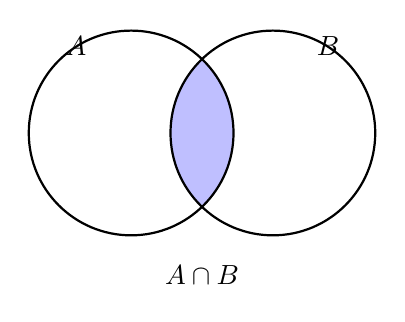
\begin{tikzpicture}
  \begin{scope}
    \clip (-0.9, 0) circle (1.3);
    \fill[blue!25] (0.9, 0) circle (1.3);
  \end{scope}
  \draw[thick] (-0.9, 0) circle (1.3);
  \draw[thick] (0.9, 0) circle (1.3);
  \node at (-1.6, 1.1) {$A$};
  \node at (1.6, 1.1) {$B$};
  \node at (0, -1.8) {$A \cap B$};
\end{tikzpicture}
\end{center}

\begin{definition}[Union]
The \emph{union}\index{union@$\cup$ (union)} of two sets $A$ and $B$ is the set of elements in either $A$ or $B$:
$A \cup B :=  \{ x \mid x \in A \text{ or } x \in B\}$.
\end{definition}

\begin{center}
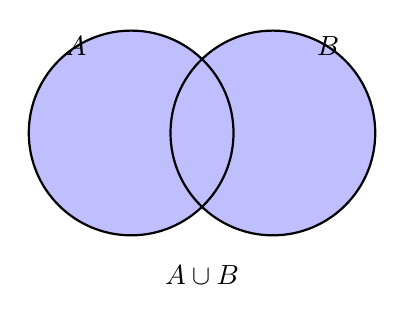
\begin{tikzpicture}
  \fill[blue!25] (-0.9, 0) circle (1.3);
  \fill[blue!25] (0.9, 0) circle (1.3);
  \draw[thick] (-0.9, 0) circle (1.3);
  \draw[thick] (0.9, 0) circle (1.3);
  \node at (-1.6, 1.1) {$A$};
  \node at (1.6, 1.1) {$B$};
  \node at (0, -1.8) {$A \cup B$};
\end{tikzpicture}
\end{center}

\begin{definition}[Subset]
Given sets $A$ and $B$, we say $A$ is a \emph{subset}\index{subset} of $B$, written $A \subseteq B$, when every element of $A$ is also an element of $B$.
\end{definition}

\begin{definition}[Set Difference]
The \emph{difference}\index{set!difference} of sets $A$ and $B$, written $A \setminus B$, is the set of elements in $A$ that are not in $B$:
$A \setminus B := \{x \mid x \in A \text{ and } x \notin B\}$.
\end{definition}

\begin{center}
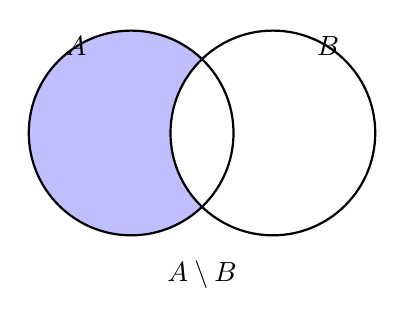
\begin{tikzpicture}
  \begin{scope}
    \clip (-0.9, 0) circle (1.3);
    \fill[blue!25] (-3, -2) rectangle (3, 2);
    \fill[white] (0.9, 0) circle (1.3);
  \end{scope}
  \draw[thick] (-0.9, 0) circle (1.3);
  \draw[thick] (0.9, 0) circle (1.3);
  \node at (-1.6, 1.1) {$A$};
  \node at (1.6, 1.1) {$B$};
  \node at (0, -1.8) {$A \setminus B$};
\end{tikzpicture}
\end{center}

\begin{definition}[Complement]
Given a universal set $U$ that contains all elements under discussion, the \emph{complement}\index{set!complement} of $A$, written $\overline{A}$, is $U \setminus A = \{x \mid x \in U \text{ and } x \notin A\}$.
\end{definition}

\begin{center}
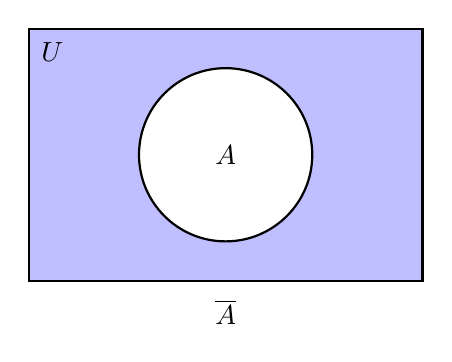
\begin{tikzpicture}
  \fill[blue!25] (-2.5, -1.6) rectangle (2.5, 1.6);
  \fill[white] (0, 0) circle (1.1);
  \draw[thick] (-2.5, -1.6) rectangle (2.5, 1.6);
  \draw[thick] (0, 0) circle (1.1);
  \node at (-2.2, 1.3) {$U$};
  \node at (0, 0) {$A$};
  \node at (0, -2.0) {$\overline{A}$};
\end{tikzpicture}
\end{center}

The complement only makes sense relative to some agreed-upon universe $U$. When we write $\overline{A}$ we're implicitly assuming everyone knows what $U$ is.

A quick notation warning: you'll also see $A^c$\index{complement!notation $A^c$} used for the complement of $A$, particularly in Lean and in the Natural Number Game. The overline and the superscript-$c$ mean the same thing; the choice is a matter of typographic convenience.

\begin{sidebar}{universes, then and now}
The phrase ``universal set'' is doing more work than it lets on. Early set theorists---Cantor, Frege---were happy to talk about \emph{the} universe: the set of absolutely everything. That ran aground on \emph{Russell's paradox}\index{Russell's paradox}: consider the ``set'' of all sets that don't contain themselves. Does it contain itself? Either answer contradicts itself. The moral was that not every predicate carves out a set. Modern axiomatic set theory (ZFC) fixes this by only letting you form $\{x \in S \mid P(x)\}$ relative to some \emph{already-existing} set $S$---exactly the ``subset with a predicate'' construction we've been using. There is no set of all sets in ZFC, so the phrase ``universe $U$'' in the definition of complement is always a stand-in for ``some large enough set we've agreed on for this discussion.''

Category theorists, who genuinely do want to talk about ``all groups'' or ``all topological spaces,'' cope with this by working inside a \emph{Grothendieck universe}\index{Grothendieck universe}---a set big enough to pretend it's everything, while technically sitting inside an even bigger one.

Type theory faces the same problem from a different angle. If you try to have a single type \texttt{Type} that contains all types, including itself, you run into Girard's paradox---a type-theoretic cousin of Russell's. Systems like Coq, Agda, and Lean solve this with a \emph{universe hierarchy}\index{universe hierarchy}: \texttt{Type 0} contains ordinary types, \texttt{Type 1} contains \texttt{Type 0}, and so on up. In practice you rarely see the indices because the elaborator figures them out for you (``universe polymorphism''), but they're always there in the background, preventing the self-referential collapse.

So when these notes say ``universe'' we mean something weaker than a god's-eye view of everything. It just means: a context---a set, a type, a level---big enough to contain what we're talking about today.
\end{sidebar}

\begin{definition}[Disjoint]
Two sets $A$ and $B$ are \emph{disjoint}\index{disjoint} if they share no elements: $A \cap B = \emptyset$.
\end{definition}

Next is something that seems obvious but is incredibly important and---in the history of mathematics---quite divisive: equality of sets.

Two sets are equal exactly when $A \subseteq B$ and $B \subseteq A$, in other words when the two sets have \emph{exactly} the same elements.

This has a couple of implications. First, there's no sense of \emph{ordering} in sets: $\{a,b,c\} = \{c,b,a\} = \{c,a,b\}$. Second, it doesn't matter how you build the sets. You could get the ``set of natural numbers divisible by four'' either as $\{x \mid x \in \mathbb{N}, x \mathbin{\%} 4 = 0\}$ or as a two-step process: first get the even numbers $E = \{x \mid x \in \mathbb{N}, x \mathbin{\%} 2 = 0\}$ and then filter as $\{x \mid x \in E, x \mathbin{\%} 4 = 0\}$. Either way, you get the ``same'' set because they have the same elements.

This is called \emph{extensional} equality\index{extensional equality}, that is equality because the two things look the same from ``the outside''.

I want to hint at why this is a useful yet \emph{controversial} definition by asking a simple question: when are two programs the same? Is producing the same output for the same input enough to call the programs the same? Why or why not?

The alternative is \emph{intensional} equality\index{intensional equality}, where two things are equal only if they're defined or constructed the same way. Consider the sets $\{x \mid x \text{ is even and } x < 10\}$ and $\{2, 4, 6, 8\}$. These are extensionally equal---they have exactly the same elements. But intensionally they're different: one is defined by a predicate, the other by enumeration. The ``recipes'' are different even though the ``dishes'' come out the same.

This is exactly the question with programs: two programs that produce the same output for every input are extensionally equal. But they might use completely different algorithms, have different performance characteristics, different memory usage. Are they ``the same program''? An extensionalist says yes; an intensionalist says no.

For sets, we're choosing the extensional view in this course---two sets with the same elements are the same set, period. But be aware that this is a choice, and in some areas of computer science and mathematics (particularly type theory and constructive mathematics), intensional equality is the default. The difference becomes important when you care not just about \emph{what} something computes but \emph{how} it computes it. We'll come back to this question---what \emph{should} count as ``the same''?---in the intermezzo ``What Does It Mean for Things to Be `The Same'?'' after Module~6.

One more consequence of extensional equality that's worth making explicit: \emph{duplicates don't count}. The set $\{2, 2, 2, 2\}$ is the same as the set $\{2\}$ because they have the exact same elements---the number 2 and nothing else. Writing 2 four times doesn't somehow put four copies of it in the set. Sets don't work like arrays.

\begin{definition}[Cardinality]
The \emph{cardinality}\index{cardinality} of a finite set $A$, written $|A|$, is the number of \emph{distinct} elements in $A$.
\end{definition}

For example:
\begin{itemize}
  \item $|\{a, b, c\}| = 3$
  \item $|\{2, 2, 2, 2\}| = |\{2\}| = 1$
  \item $|\{\}| = 0$ (the empty set has no elements). The set with no elements, written $\{\}$ or $\emptyset$, is called the \emph{empty set}\index{empty set}.
\end{itemize}

One that trips people up: what about $\{0, \{0\}\}$? This set has two elements: the number $0$ and the set $\{0\}$. These are different things! One is a number and the other is a set that \emph{contains} a number. So $|\{0, \{0\}\}| = 2$. Don't confuse an element with a set containing that element---$0$ and $\{0\}$ are not the same thing, just like a box is not the same thing as what's inside it.\footnote{If you're a Python programmer: \texttt{0 == \{0\}} is \texttt{False}. If that seems obvious to you, good. But it's the kind of thing that causes errors on homework.}

\begin{definition}[Power Set]
The \emph{power set}\index{set!power} of a set $A$, written $\mathcal{P}(A)$, is the set of all subsets of $A$:
$\mathcal{P}(A) := \{S \mid S \subseteq A\}$.
\end{definition}

For example, $\mathcal{P}(\{1, 2\}) = \{\emptyset, \{1\}, \{2\}, \{1,2\}\}$. Notice that the power set always includes both $\emptyset$ (the empty set is a subset of everything) and $A$ itself ($A \subseteq A$).

How big is the power set? For a set with $n$ elements, $|\mathcal{P}(A)| = 2^n$. Each element of $A$ is either in a given subset or not---two choices per element, so $2 \times 2 \times \cdots \times 2 = 2^n$ total subsets. We'll see where this $2^n$ comes from more deeply in the next chapter.

The final concept to discuss with sets is another operation: the \emph{product} of sets. Epp's approach is to derive products from more basic set operations, which is a worthwhile exercise and worth reading once. In these notes, we'll instead take tuples as a basic building block, which is more common in the kind of foundational mathematics you'll encounter as a computer scientist.

You've seen tuples before: coordinates! $(3,4)$ is three units in the x-direction, four units in the y-direction. Tuples are, in a sense, the opposite of sets. They have \emph{order} and a \emph{fixed size}. If you want an analogy, think of arrays in C/C++: you can have arrays of arbitrary size but any \emph{given} array has a size that you decided on in advance.

\begin{definition}[Cartesian Product]
The \emph{Cartesian product}\index{Cartesian product} of sets $A$ and $B$ is the set of all tuples\index{tuple} made from $A$ and $B$:
$A \times B = \{(a,b) \mid a \in A, b \in B\}$.
\end{definition}

With all of that, we can move on to the last topic of this first module: functions and relations.

\section{Functions and relations}

As with the last section we'll diverge a little from Epp here.

\begin{definition}[Function]
A \emph{function}\index{function} $f$ from a set $A$ to a set $B$, denoted $f : A \rightarrow B$, is an assignment that sends \emph{every} element of $A$ to \emph{exactly one} element of $B$. That is, every $a \in A$ has an output $f(a) \in B$, and if $f(a) = b$ and $f(a) = c$ then $b = c$.
\end{definition}

There are two requirements packed into this definition: \emph{totality} (every element of $A$ must have an output) and \emph{uniqueness} (each element of $A$ maps to exactly one element of $B$, not two or more). If we drop the totality requirement---allowing some elements of $A$ to have no output---we get a \emph{partial function}\index{partial function}. Partial functions come up naturally in computer science (think of a program that might crash or loop forever on certain inputs), but unless we say ``partial'' explicitly, ``function'' always means the total version.

Epp defines a function as a subset of $A \times B$. This is related, but in general ``a function as a gadget that assigns elements of one set to another'' and ``the subset of tuples in $A \times B$ that describes the action of the function'' are two different concepts that we need to keep distinct. This connects back to the question about when two programs are the same that we raised in the previous section.

It's important to note that functions in mathematics include both things we know how to calculate, like $f(x) = x +1$, and things we don't. For example, consider a function that maps each C program implementing a function from integers to integers to the smallest input that doesn't cause it to go into an infinite loop, if one exists. That's a weird partial function, but it's a well-defined assignment, and it's definitely not something you can calculate.

\subsection*{Composing functions}

Functions are more useful once we can chain them together. If $f$ takes us from $A$ to $B$ and $g$ takes us from $B$ to $C$, there is an obvious combined function that takes us from $A$ all the way to $C$: apply $f$, then apply $g$.

\begin{definition}[Composition]
Given functions $f : A \to B$ and $g : B \to C$, their \emph{composition}\index{composition of functions} is the function $g \circ f : A \to C$ defined by
\[
  (g \circ f)(a) \;=\; g(f(a))
\]
for every $a \in A$.
\end{definition}

Read $g \circ f$ as ``$g$ after $f$.'' The order is backwards from how you say it in English (``first $f$, then $g$'') but it matches the order you'd evaluate it in: to compute $(g \circ f)(a)$ you write down $g(f(a))$, and now the $f$ is closer to the $a$, which is closer to where the computation starts.

\begin{center}
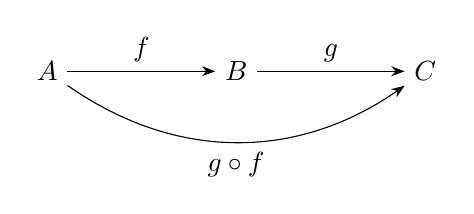
\begin{tikzpicture}[node distance=2.4cm, >=Stealth]
  \node (A) {$A$};
  \node (B) [right of=A] {$B$};
  \node (C) [right of=B] {$C$};
  \draw[->] (A) -- node[above] {$f$} (B);
  \draw[->] (B) -- node[above] {$g$} (C);
  \draw[->, bend right=35] (A) to node[below] {$g \circ f$} (C);
\end{tikzpicture}
\end{center}

For every set $A$ there is a trivial-looking function we'll use constantly: the \emph{identity function}\index{identity function} $\mathrm{id}_A : A \to A$, defined by $\mathrm{id}_A(a) = a$. It does nothing to its input. The reason it earns a name is that it is the neutral element for $\circ$:

\begin{itemize}
  \item \textbf{Left identity:} $\mathrm{id}_B \circ f = f$ for every $f : A \to B$.
  \item \textbf{Right identity:} $f \circ \mathrm{id}_A = f$ for every $f : A \to B$.
  \item \textbf{Associativity:} $(h \circ g) \circ f = h \circ (g \circ f)$ whenever the types line up.
\end{itemize}

Each of these is checked the same way: apply both sides to an arbitrary input $a$ and observe you get the same output. For the associativity law, for instance, both sides send $a$ to $h(g(f(a)))$.

In Python, $\circ$ is a one-liner:
\begin{lstlisting}
def compose(g, f):
    return lambda x: g(f(x))
\end{lstlisting}

This little operation will reappear in surprising places as the course goes on. It is the way transitive implications chain in Module~3 (from $A \Rightarrow B$ and $B \Rightarrow C$ you get $A \Rightarrow C$), it is what makes the invertible functions on a set into a group in Module~5, and it shows up as a proof-combining rule in the Curry--Howard intermezzo. Whenever you see ``do this, then do that, and the types line up,'' $\circ$ is hiding in the background.

\begin{definition}[Relation]
A \emph{relation}\index{relation} between sets $A$ and $B$ is a subset of $A \times B$ --- a collection of pairs $(a, b)$ recording which elements of $A$ are related to which elements of $B$. Unlike a function, a relation allows an element of $A$ to be related to zero, one, or many elements of $B$.
\end{definition}

We've already seen one important relation: $\subseteq$ is a relation on sets. You can have $A \subseteq B$ and $A \subseteq C$ without $B$ and $C$ being the same, because $\{1\} \subseteq \{1,2\}$ and $\{1\} \subseteq \{1,3\}$.

A few more examples of relations you already know: equality on a set (is $a$ the same as $b$?), ``less than'' on the integers ($3 < 5$ but not $5 < 3$), and ``is a prerequisite of'' on courses (CS 250 is a prerequisite of CS 251, but not the other way around).

When we have a relation $R$ on a single set $A$ (that is, $R$ relates elements of $A$ to other elements of $A$), we can ask what \emph{properties} it has. Three come up constantly.

\begin{definition}[Reflexive]
A relation $R$ on a set $A$ is \emph{reflexive}\index{reflexive} if every element is related to itself: for all $a$ in $A$, $a \, R \, a$.
\end{definition}

\begin{definition}[Symmetric]
A relation $R$ on a set $A$ is \emph{symmetric}\index{symmetric} if whenever $a$ is related to $b$, then $b$ is related to $a$: for all $a, b$ in $A$, if $a \, R \, b$ then $b \, R \, a$.
\end{definition}

\begin{definition}[Transitive]
A relation $R$ on a set $A$ is \emph{transitive}\index{transitive} if relations chain: for all $a, b, c$ in $A$, if $a \, R \, b$ and $b \, R \, c$, then $a \, R \, c$.
\end{definition}

\begin{definition}[Equivalence Relation]
A relation that is reflexive, symmetric, \emph{and} transitive is called an \emph{equivalence relation}\index{equivalence relation}.
\end{definition}

Equality is the canonical equivalence relation---it's reflexive ($a = a$), symmetric ($a = b$ implies $b = a$), and transitive ($a = b$ and $b = c$ implies $a = c$). We'll see other equivalence relations later in the course, such as modular congruence.

Which properties do our other examples satisfy? ``Less than'' on the integers is transitive ($a < b$ and $b < c$ implies $a < c$) but not reflexive ($3 \not< 3$) and not symmetric ($3 < 5$ but $5 \not< 3$). The subset relation $\subseteq$ is reflexive ($A \subseteq A$) and transitive but not symmetric ($\{1\} \subseteq \{1,2\}$ but $\{1,2\} \not\subseteq \{1\}$).

\section{Summary and looking ahead}

\begin{keytakeaway}
  \item A \emph{set} is an unordered, duplicate-free collection of elements; equality is \emph{extensional} (two sets are equal when they have the same elements).
  \item Standard set operations: union $\cup$, intersection $\cap$, difference $\setminus$, complement $\overline{\cdot}$, Cartesian product $\times$, power set $\mathcal{P}$. The power set of an $n$-element set has $2^n$ elements.
  \item A \emph{function} $f : A \to B$ is a total, single-valued assignment from $A$ to $B$. Dropping totality gives a \emph{partial function}. Functions \emph{compose}: given $f : A \to B$ and $g : B \to C$ there is $g \circ f : A \to C$, with the identity function $\mathrm{id}$ as a two-sided unit.
  \item A \emph{relation} between $A$ and $B$ is any subset of $A \times B$. Relations on a single set can be \emph{reflexive}, \emph{symmetric}, or \emph{transitive}; a relation with all three properties is an \emph{equivalence relation}.
\end{keytakeaway}

\begin{summarybox}
\textbf{What we built this module.} We laid the vocabulary groundwork for the rest of the course. Sets and functions are the universe inside which we'll do everything else; the definitions of reflexive, symmetric, and transitive relations are the pattern we'll meet over and over (equivalence relations in Module 6, modular congruence, the $\leq$ ordering, the Curry--Howard correspondence in the intermezzo).

\medskip
\textbf{Looking ahead.} The short chapter that immediately follows, ``How to Write a Proof,'' collects practical advice on the prose style every proof in the book expects. Re-read it as you do the exercises below. Module~2 then starts the formal logic thread: we'll define propositional logic with a BNF grammar and give its truth-table semantics. That logic has just two values---true and false---so we can check everything exhaustively, which makes it a clean place to build habits before we add quantifiers (Module~4) and proofs-on-infinite-data (Module~8). Along the way, the intermezzo after this module (``Cardinality and Function Spaces'') uses the set and function vocabulary from here to show that some infinities are bigger than others---a real surprise that's worth the detour.
\end{summarybox}

\section{Exercises}

The exercises below are organized into four tiers. The \textbf{warm-ups} are short, mechanical checks on the definitions---do them all. The \textbf{standard} problems are closer to what you'll see on an assignment or exam. The \textbf{challenge} problems ask you to stitch several ideas together and are the ones most worth discussing with a study partner. The \textbf{connection} problems point outward---to programming, to the intermezzo on cardinality, or to later modules. Solutions for all of these are in the appendix, but resist the temptation to look until you've tried.

\subsection*{Warm-up}

\textbf{Exercise 1.}\label{ex:m1:1} Let $A = \{1, 2, 3, 4\}$ and $B = \{3, 4, 5, 6\}$. Compute $A \cap B$, $A \cup B$, $A \setminus B$, and $|A \times B|$.

\bigskip
\noindent\textbf{Exercise 2.}\label{ex:m1:2} What is $|\{1, \{1\}, \{1, \{1\}\}\}|$? Be careful---count distinct elements.

\bigskip
\noindent\textbf{Exercise 3.}\label{ex:m1:3} Rewrite the set $\{n \mid n \in \mathbb{N},\; n^2 < 20\}$ by listing its elements explicitly (``roster notation''). Then do the same for $\{n \mid n \in \mathbb{Z},\; -3 \leq n < 3\}$.

\bigskip
\noindent\textbf{Exercise 4.}\label{ex:m1:4} Let $S = \{1, 2, \{1\}, \{1, 2\}\}$. For each of the following, say whether it is true, false, or a type error (``type error'' means the claim doesn't even make sense---e.g., asking whether a number is a subset of another number):
\begin{enumerate}[label=(\alph*)]
  \item $1 \in S$
  \item $\{1\} \in S$
  \item $\{1\} \subseteq S$
  \item $\{1, 2\} \in S$
  \item $\{1, 2\} \subseteq S$
  \item $\{\{1\}\} \subseteq S$
  \item $2 \subseteq S$
\end{enumerate}

\bigskip
\noindent\textbf{Exercise 5.}\label{ex:m1:5} List all eight elements of $\mathcal{P}(\{a, b, c\})$ and verify that there are $2^3$ of them. Then list all six elements of $\{a, b\} \times \{1, 2, 3\}$.

\subsection*{Standard}

\textbf{Exercise 6.}\label{ex:m1:6} For each of the following relations on $\mathbb{Z}$, determine whether it is reflexive, symmetric, and/or transitive: (a) $a\, R\, b$ iff $a + b$ is even; (b) $a\, R\, b$ iff $a \leq b$; (c) $a\, R\, b$ iff $|a - b| \leq 1$.

\bigskip
\noindent\textbf{Exercise 7.}\label{ex:m1:7} For each of the following ``assignments'' from $\mathbb{R}$ to $\mathbb{R}$, decide whether it is a function (in the total, single-valued sense of the definition in this module). If it isn't, say which requirement fails---totality or uniqueness---and give a witness. If it is, say so explicitly.
\begin{enumerate}[label=(\alph*)]
  \item $f(x) = 1/x$.
  \item $f(x) = \sqrt{x}$ (taking only the non-negative square root).
  \item The relation $\{(x, y) \mid y^3 = x\}$, viewed as an assignment $x \mapsto y$.
  \item The relation $\{(x, y) \mid y^2 = x\}$, viewed as an assignment $x \mapsto y$.
\end{enumerate}

\bigskip
\noindent\textbf{Exercise 8.}\label{ex:m1:8} Prove the distributive law $A \cap (B \cup C) = (A \cap B) \cup (A \cap C)$ by showing both containments. That is, show $A \cap (B \cup C) \subseteq (A \cap B) \cup (A \cap C)$ and vice versa, each by picking an arbitrary element of the left-hand side and arguing that it must be in the right-hand side. Use the ``state goal, introduce variable, justify every step'' advice from the ``How to Write a Proof'' chapter.

\bigskip
\noindent\textbf{Exercise 9.}\label{ex:m1:9} Prove or disprove: for all sets $A$ and $B$, if $A \subseteq B$ then $\mathcal{P}(A) \subseteq \mathcal{P}(B)$. (Reminder: to prove an implication about sets, start by assuming the hypothesis and by picking an arbitrary element of the set whose containment you want to show.)

\bigskip
\noindent\textbf{Exercise 9b.}\label{ex:m1:9b} (Composition.) Let $f : \mathbb{Z} \to \mathbb{Z}$ send $n \mapsto n+1$ and let $g : \mathbb{Z} \to \mathbb{Z}$ send $n \mapsto 2n$. Compute $g \circ f$ and $f \circ g$ as closed-form expressions, and confirm that they are \emph{not} the same function. Then verify, for an arbitrary $n$, the associativity law $((f \circ f) \circ g)(n) = (f \circ (f \circ g))(n)$.

\subsection*{Challenge}

\textbf{Exercise 10.}\label{ex:m1:10} Let $A$ and $B$ be finite sets. Prove that
\[
  |A \cup B| = |A| + |B| - |A \cap B|.
\]
Give a plain-English argument (``every element of $A \cup B$ is counted \ldots''). This is your first taste of \emph{inclusion--exclusion}, which generalizes to arbitrary finite unions and is one of the foundational tools of combinatorics.

\bigskip
\noindent\textbf{Exercise 11.}\label{ex:m1:11} A \emph{relation on $A$} is a subset of $A \times A$, so relations on $A$ are themselves elements of the power set $\mathcal{P}(A \times A)$. If $|A| = n$, how many distinct relations are there on $A$? How many are reflexive? (Hint for the second part: a reflexive relation \emph{must} contain all $n$ diagonal pairs, and is free to include or exclude each of the remaining pairs.)

\bigskip
\noindent\textbf{Exercise 12.}\label{ex:m1:12} Here is a classic bad argument: ``Symmetry and transitivity together force reflexivity. After all, if $a\, R\, b$, then by symmetry $b\, R\, a$, and so by transitivity $a\, R\, a$.'' Find the flaw---this really is a common error---and then exhibit a concrete relation on $\{1, 2, 3\}$ that is symmetric and transitive but \emph{not} reflexive. What additional assumption would you need for the argument to go through?

\subsection*{Connection}

\textbf{Exercise 13.}\label{ex:m1:13} (Programming.) Write a Python function \texttt{cartesian(xs, ys)} that takes two lists and returns the Cartesian product as a list of tuples, \emph{without} using \texttt{itertools.product}. Test it on \texttt{cartesian([1,2],\ ['a','b','c'])} and verify it produces the same six tuples you listed by hand in Exercise~\ref{ex:m1:5}. Then answer: if \texttt{xs} has length $m$ and \texttt{ys} has length $n$, how many element comparisons does your implementation do?

\bigskip
\noindent\textbf{Exercise 14.}\label{ex:m1:14} (Intermezzo pointer.) The intermezzo after this module, ``Cardinality and Function Spaces,'' is about counting functions between finite sets. As a warm-up for it: how many functions are there from $\{a, b, c\}$ to $\{0, 1\}$? List them all as tables. Can you see why the answer is $2^3$ and not $3^2$? (Which set plays the role of ``exponent''?)

\bigskip
This has been a foundational week: sets, tuples, functions, relations, and (in the short chapter that follows) the prose style expected of every proof in the book. Those are the vocabulary we'll use for the rest of the course. In the next module we start doing \emph{logic}.

\end{document}
